\documentclass{article}
\usepackage[utf8]{inputenc}
\usepackage[margin=1in]{geometry}

%==========================================================

\usepackage{amsmath,amssymb,amsfonts,amsthm}
\usepackage{scrlayer-scrpage}
\usepackage{tikz}
\usepackage{algorithm}
\usepackage{algpseudocode}
\usepackage{listings}
\usepackage{xcolor}
\usepackage{color}
\usepackage{textcomp}

%\setkomafont{section}{\huge\bfseries}

%==========================================================

\pagestyle{scrheadings}

\title{Aufgabe 1\\Wörter aufräumen}
\author{Tassilo Tanneberger}

\newcommand{\linia}{\rule{\linewidth}{1pt}}
\makeatletter
\renewcommand{\maketitle}{\begin{center}
\Huge \@title\end{center}
\linia\\
{\large\@author\hfill\@date\\}}

%==========================================================

\graphicspath{ {./resources/} }

%==========================================================

\definecolor{codegreen}{rgb}{0,0.6,0}
\definecolor{codegray}{rgb}{0.5,0.5,0.5}
\definecolor{codepurple}{rgb}{0.58,0,0.82}
\definecolor{backcolour}{rgb}{0.95,0.95,0.95}

\definecolor{dkgreen}{rgb}{0,0.6,0}
\definecolor{gray}{rgb}{0.5,0.5,0.5}
\definecolor{mauve}{rgb}{0.58,0,0.82}

%\lstset{frame=tb,
%  aboveskip=3mm,
%  belowskip=3mm,
%  columns=flexible,
%  basicstyle={\small\ttfamily},
%  numbers=none,
%  numberstyle=\tiny\color{gray},
%  keywordstyle=\color{blue},
%  commentstyle=\color{dkgreen},
%  stringstyle=\color{mauve},
%  breaklines=true,
%  tabsize=3,
%}

\lstset{
	language=C++,
    backgroundcolor=\color{backcolour},   
    commentstyle=\color{codegreen},
    keywordstyle=\color{magenta},
    numberstyle=\tiny\color{codegray},
    stringstyle=\color{codepurple},
    basicstyle=\ttfamily\footnotesize,
    breakatwhitespace=false,         
    breaklines=true,                 
    captionpos=b,                    
    keepspaces=true,                 
    numbers=left,                    
    numbersep=5pt,                  
    showspaces=false,                
    showtabs=false, 
    frameround=ffff,                 
    tabsize=3,
    columns=flexible,
    showstringspaces=false
}

%==========================================================

\begin{document}

\maketitle


\section*{Theorie \& Lösungsidee}

Die Grundidee ist ziemlich simpel: wir suchen alle Wörter, die zu einem Lückenwort passen, heraus und sammeln diese in einer Liste. Das führen wir für jedes Lückenwort durch. Danach beginnen wir mit dem Lückenwort, welches die wenigsten passenden Wörter hat. Wir führen folgenden Schritt für jedes passende Wort aus. Wir löschen das Wort einmal aus den möglichen Wörtern anderer Lückenwörter, weil das Wort nun genutzt wird. Danach beginnt der Prozess wieder bei der Suche des Lückenwortes mit minimaler Anzahl von Auswahlmöglichkeiten.

\paragraph*{Anmerkung zur mathematischen Formulierung: } $ l $ ist ein Lückenwort aus der Menge aller Lückenwörter $ L $ und $ w $ ist ein mögliches angegebenes Wort aus $ W $. Die Funktion $ \Psi (l, w) \in \lbrace 0, 1 \rbrace $ trifft eine Aussage darüber ob ein Wort $ w $ zu einen Lückenwort $ l $ zugeordnet werden kann.
\begin{align*}
	&f(l) : L \rightarrow \lbrace W \rbrace\\
	&f(l) = \lbrace w_i \in W \vert\ \Psi (l, w_i)\ i = (1, \dots, \vert W \vert ) \rbrace \\
	&f(l) \ \dots \ \textit{Alle Wörter, die zu einen gegebenen Lückenwort } l \textit{ passen}
\end{align*}

\noindent Die Funktion $ \Psi (l, w) $ schaut ob zu einem gegebenem Wort einen gegebenes Lückenwort passt. Ein nicht gesetzter Buchstabe eines Lückenwortes wird mit einem "\textunderscore "\ gekennzeichnet. Die Funktion hinter $ \Psi $ iteriert einfach über die Buchstaben in dem Wort und dem Lückenwort und vergleicht die Buchstaben. Wenn er ein "\textunderscore " \ findet wird der Buchstabe aus $ w $ ignoriert. Nur wenn jeder Buchstabe aus $ w $ mit jedem Symbol aus $ l $ übereinstimmt, wird $ 1 $ zurückgegeben. \\

\noindent $ f(l) $ spielt eine wichtige Rolle, da es alle Wörter aussortiert, die nicht zu einen gegebenen Lückenwort $ l $ passen. Somit kann man Lückenwörter priorisieren abhängig davon, wie viele Wörter noch vorhanden sind, die zu dem Lückenwort passen ( $ \vert f(l) \vert $ ). Mathematisch betrachtet ist $ f(l) $ eine Mengenfunktion.\\

\noindent Nun müssen den Algorithmus nur noch formal definieren. Ich habe den Algorithmus in zwei Funktionen gespalten. Die erste Funktion ( Find-Min-Size($W, L$) ) sucht das Lückenwort heraus, was die geringste Auswahl an passenden Wörtern hat und somit als nächstes ein Wort zugewiesen bekommt. Die zweite Funktion ( Recursive-Search($W, L, C$) ) generiert über einen Backtracking-Ansatz alle möglichen Sätze. 

\begin{algorithm}[H]
\caption{ Finden möglicher Zuordnungen }
\label{euclid}
\begin{algorithmic}[1]
	\State $ K \dots $ Lösungsmenge

	\Function{Find-Min-Size}{$W, L$}
	\State $ \lambda \dots \textsc{Min Value}$
	\State $ I \dots \textsc{Index} $
	\For{$ i = (1, \dots, \vert L \vert ) $}
		\If{ $ \vert f( l_i ) \vert < \lambda \land \vert f( l_i ) \vert \neq 0 $ }
			\State $ \lambda \gets \vert f(l_i) \vert $
			\State $ I \gets i $
		\EndIf
    \EndFor
    \State \Return { $ I $ }
	\EndFunction \\
	
	\Procedure {Recursive-Search}{$W, L, C $}
		\State $ I \gets$ Find-Min-Size($ W, L $)
		
		\If { $ \vert K_I \vert = 0 $ } \Comment{Abbruchbedingung}
			\If{ $  \vert C \vert \leftrightarrow \vert L \vert \land C \not\in K $}
				\State $ K \gets K \cup \lbrace C \rbrace $ \Comment{Mögliche Lösung gefunden}
			\EndIf
			\State \Return
		\EndIf
		
		\For{ $ w \textsc{ in } R_I $}
			\State $ P \gets W \setminus \lbrace w \rbrace $
			\State $ C \gets C \cup \lbrace w \rbrace $
			\State Recursive-Search($P, L, C $)
			\Comment{ Rekursiver Neuaufruf }
		\EndFor
		
	\EndProcedure
\end{algorithmic}
\end{algorithm}

Nehmen wir ein kleines Beispiel und führen den Algorithmus damit durch.

\begin{itemize}
	\item Lückenwörter $ L = \lbrace "M \textunderscore h \textunderscore"," \textunderscore \textunderscore \textunderscore \textunderscore \textunderscore ", " \textunderscore \textunderscore \textunderscore \textunderscore " \rbrace$
	\item Wörter $ W = \lbrace "Meer", "nicht", "Mehr" \rbrace $ 
\end{itemize}

Von den gegebenen Lückenwörtern ist nur $ l_3 = "\textunderscore \textunderscore \textunderscore \textunderscore" $ uneindeutig: $ \vert f("\textunderscore \textunderscore \textunderscore \textunderscore ") \vert = 2 $ (Verzweigung im Lösungsbaum). 
Somit wird $ l_3 $ als letztes ein Wort zugewiesen. Eine Verzweigung entsteht dann, wenn der Algorithmus sich nicht sicher ist, welches Wort er nun einsetzten soll: $ \vert f(l) \vert > 1$. 

\begin{tikzpicture}%[sibling distance=10em,
  % every node/.style = {shape=rectangle, rounded corners, draw, align=center, top color=white, bottom color=blue!20}]]
  \node { $ \lbrace \rbrace $ }
    child { node { $ \lbrace "Mehr" \rbrace$ }
    child { node {$ \lbrace "Meer", "nicht" \rbrace $}
    child { node {$ \lbrace "Mehr", "nicht", "Meer" \rbrace $ } } }
 };
 
   \node[text width=9cm] at (8,0) {$ f("M \textunderscore h \textunderscore") = \lbrace "Mehr" \rbrace $\\$ W = \lbrace "Meer", "nicht", "Mehr" \rbrace $};
 
    \node[text width=9cm] at (8,-1.5) {$ f(" \textunderscore \textunderscore \textunderscore \textunderscore \textunderscore ") = \lbrace "nicht" \rbrace $\\$ W = \lbrace "Meer", "nicht" \rbrace $};
    
    \node[text width=9cm] at (8,-3) {$ f(" \textunderscore \textunderscore \textunderscore \textunderscore ") = \lbrace "Meer" \rbrace $\\$ W = \lbrace "Meer"\rbrace $};
    
    \node[text width=9cm] at (8,-4.5) {$ W = \lbrace \rbrace $};
\end{tikzpicture}

\paragraph{Weitere Ideen}
Für eine besonders ambitionierte Lösung kann man auch die Funktion $ \Psi $ mit der Levenshtein-Distanz $d(l, w)$ ersetzen. Das würde den Vorteil mit sich bringen, dass man nicht mehr schaut ob ein gegebenes Wort auf ein Lückenwort passt, sondern wie ähnlich es dem Lückenwort ist.
\vspace{0.5cm}

\section*{Implementierung}

Das Programm wurde in C++ umgesetzt. In diesem Abschnitt werden wir ausgewählte Quellcodestücke näher betrachten.
\subsubsection*{Code-Beispiel 1.)}
\lstset{language=C++}
\begin{lstlisting}[language=C++]
unsigned int index = 0;
unsigned int min_value;

min_value = std::numeric_limits<unsigned int>::max();
for (unsigned int i = 0; i < possible_words.size(); i++) {
	if (min_value > possible_words.at(i).size() and not possible_words.at(i).empty()) {
		min_value = possible_words.at(i).size();
		index = i;
	}
}
\end{lstlisting}
Code-Beispiel 1 ist die Umsetzung der Funktion $Find-Min-Size(W, L)$, die aus dem Pseudo-Code bekannt ist. Wir benötigen zwei Variablen: \verb| index | speichert, welches Lückenwort als nächstes besetzt werden muss und die Variable \verb| min_value | sagt aus, wie viele Wörter in das Lückenwort passen, welches durch \verb| index | referenziert wird.

\subsubsection*{Code-Beispiel 2.)}
\lstset{language=C++}
\begin{lstlisting}[language=C++]
for (const auto &word : possible_words.at(index)) {
		  // implicit deep copy 
        std::vector<std::vector<std::string>> possible_words_copy = possible_words;
		
		  // removing word from possible_words_copy
        for (std::vector<std::string> &vec : possible_words_copy) {
            auto iter_index = std::find(vec.begin(), vec.end(), word);
            if (iter_index != vec.end()) {
                vec.erase(iter_index);
                break;
            }
        }

        std::vector<std::string> result_copy = result; // making a deep copy implicitly 
        result_copy.reserve(words_.size()); // already allocating memory 
        result_copy[index] = word; // pushing the newly assigned word into the result container

        recursive(possible_words_copy, result_copy);
}
\end{lstlisting}
Das ist das Kernstück des Algorithmus. Hier entsteht einmal die Baumstruktur durch die For-Schleife, und auch der rekursive Neu-Aufruf ist in diesem Code-Beispiel untergebracht. Dieses Codesegment beginnt damit über alle möglichen Wörter für ein gewisses Lückenwort zu iterieren. In der Implementation wird $ W $ als \verb|possible_words| bezeichnet und ist eine zweidimensionale Liste. Dabei repräsentiert \verb|index| ein bestimmtes Lückenwort und die dazu gehörige Liste entspricht der oben definierten Funktion $ f(l) $. Die Zeilen 5 bis 10 machen nichts anderes als das aktuelle Wort aus \verb|possible_words_copy| zu entfernen. Danach fügen wir das aktuelle Wort dem Result-Container $ C $ hinzu. Jetzt haben wir $ W $ und $ C $ jeweils verändert und somit können wir die nächste Ebene des Baumes evaluieren.

\newpage
\subsubsection*{Code-Beispiel 3.)}
\lstset{language=C++}
\begin{lstlisting}[language=C++]
auto MatcherClass::match() -> result {
    /*!
     * The idea here is that we generate list of words that would fit that position and than start with the smallest
     * list filling the string and removing the word from all list that contain the word
     */
    std::vector<std::string> result(words_.size());
    std::vector<std::vector<std::string>> possible_words;

    unsigned int iterator = 0;
    for (const auto &pattern: text_) {
        possible_words.emplace_back();
        for (const auto &word: words_) {
            if (MatcherClass::pattern_match(pattern, word)) {
                possible_words.at(iterator).push_back(word);
            }
        }
        if (possible_words.at(iterator).empty()) {
            return failure; // a pattern word has 0 fitting words therefore this is not solveable
        }

        iterator++;
    }
    recursive(possible_words, result);

    return (corrected_text_.empty()) ? failure : success;
}
\end{lstlisting}
Durch den Konstruktor der \verb|MatcherClass| wurden die Variablen \verb|text_| und \verb|words_| bereits gesetzt. In den Zeilen 9 bis 22 wird \verb|possible_words_|  (formal $ f(l) $) erzeugt. Dabei wird über die Lückenwörter aus dem Lückentext iteriert und alle dazu passenden Wörter in einer Liste gesammelt.

\subsection*{Vorverarbeitung und Nachverarbeitung}

Die Nutzereingabe besteht aus zwei Zeichenketten, aus denen zuerst alle Sonderzeichen wie "?", "!", ".", "," entfernt werden. Danach werden diese Strings in \verb|std::vector<std::string>| gespalten, wobei Leerzeichen als Trennzeichen fungieren. Diese beiden Listen werden dann dem Algorithmus (\verb|MatcherClass|) übergeben. Dieser produziert eine bestimmte Menge an Listen aus Zeichenketten. Die Listen müssen nun in der Nachverarbeitung wieder zu Zeichenketten zusammengesetzt werden. Zudem werden hier auch wieder die Sonderzeichen eingefügt.

\newpage

\section*{Beispiel-Druchläufe}

\begin{figure}[h]
	\center
	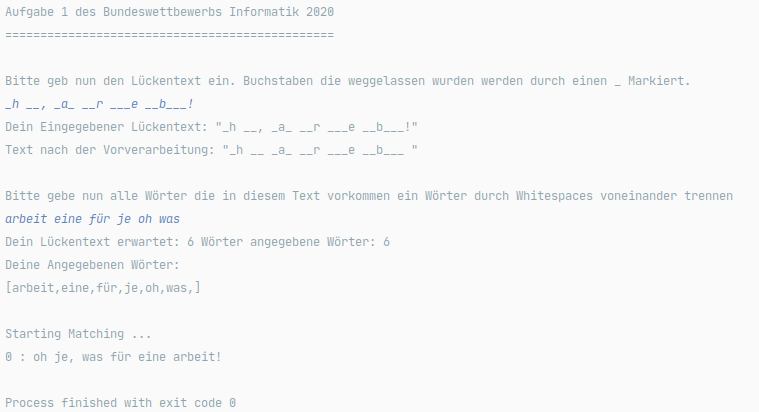
\includegraphics[width=1.0\textwidth]{aufgabe_example_ver1.png}
	\caption{Konsolen-Output des Programms mit dem Beispiel aus der Aufgabenstellung (Rätsel 1)}
	
	\vspace{0.5cm}
	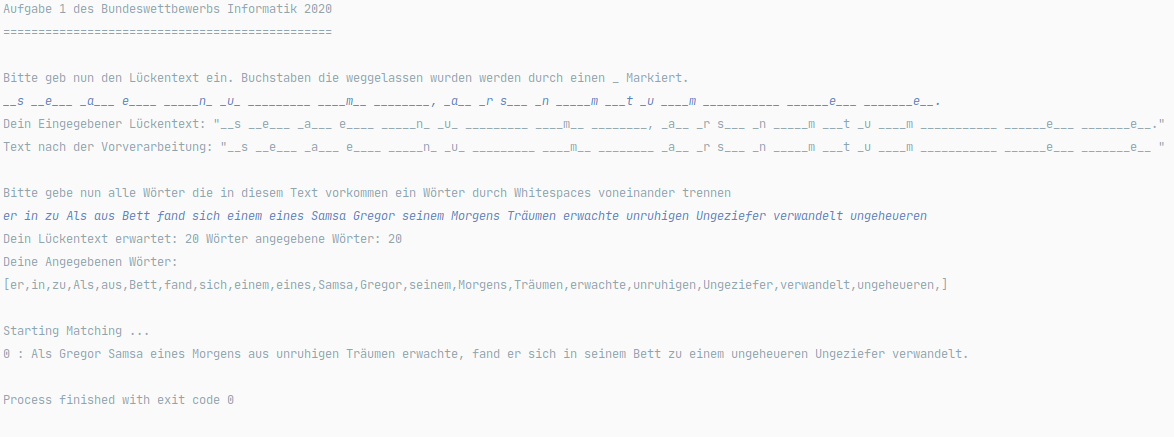
\includegraphics[width=1.0\textwidth]{aufgabe_example.png}
	\caption{Konsolen-Output des Programms mit dem Beispiel aus Rätsel 2 von der BWINF-Website}
\end{figure}




\end{document}
